\documentclass{article}
\usepackage{tikz}
\usepackage{array}
\usepackage{graphicx}
\usepackage{subfigure}
\usepackage{lscape}
\usepackage{amsmath}
\usepackage{longtable}
\usepackage{multirow}

\newcommand{\includegraphicsexempt}[2][]{\includegraphics[#1]{#2}}
\DeclareMathOperator{\Var}{var}
\DeclareMathOperator{\mean}{mean}
\DeclareMathOperator{\logit}{logit}
\renewcommand{\baselinestretch}{0.8}

\DeclareMathOperator{\nn}{n}
\DeclareMathOperator{\ii}{\psi}
\DeclareMathOperator{\cc}{\theta}

\title{Alternative Splicing in Human and Mouse}

\begin{document}
%%%%%%%%%%%%%%%%%%%%%%%%%%%%%%%%%%%%%%%%%%%%%%%%%%%%%%%%%%%%%%%%%%%%%%%%%%%%%%%%%%%%%%%%%%%%%%%%%%%%%%%%%%%%%%
\maketitle
\tableofcontents
\listoffigures
\listoftables
\clearpage

\section{Introduction}
\subsection{Definitions}
\begin{itemize}
\item Splice sites, exons, and introns are classified by usage and level
\begin{center}
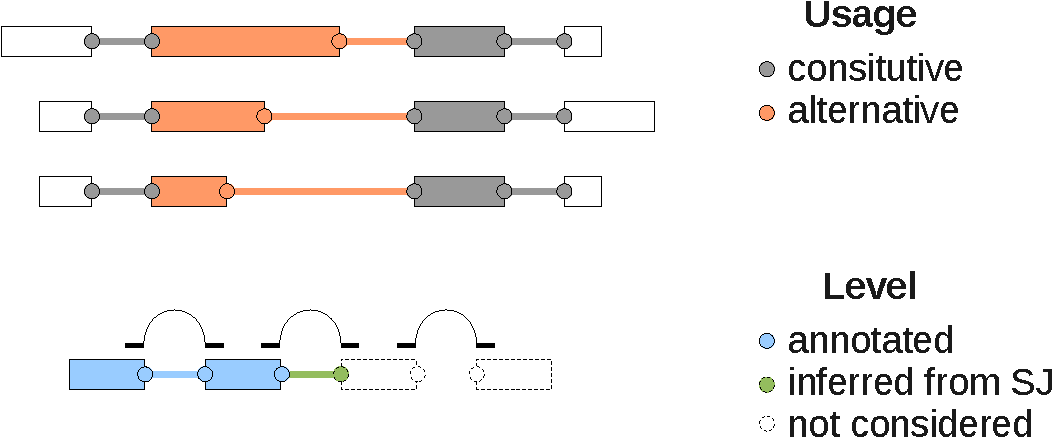
\includegraphics[height=5cm]{Latex/main_legend_1.pdf}
\end{center}
\item Only {\bf internal} splice sites, exons, and introns
\item biotypes :
\begin{itemize}
\item protein coding
\item pseudogene = pseudogene + polymorphic/processed/unprocessed pseudogene
\item lncRNA    = lincRNA + processed transcript
\item other (none of the above)
\end{itemize}
\end{itemize}
\clearpage
%%%%%%%%%%%%%%%%%%%%%%%%%%%%%%%%%%%%%%%%%%%%%%%%%%%%%%%%%%%%%%%%%%%%%%%%%%%%%%%%%%%%%%%%%%%%%%%%%%%%%%%%%%%%%%
\subsection{Splice sites}
\subsubsection{Attributes}
\begin{itemize}
\item chromosome, position, strand
\item gene
\item boundary $\in\{$acceptor, donor$\}$ NB: start and stop are not included
\item biotype $\in\{$protein coding, pseudogene, lncRNA, other$\}$
\item level $\in\{$annotated, predicted from SJ$\}$
\item usage $\in\{$alternative, constitutive$\}$
\item {\color{blue} strength}
\end{itemize}

\subsubsection{Summary stats}
\input{output/hg19.table1a.tex}
\input{output/mm9.table1a.tex}
\clearpage

%%%%%%%%%%%%%%%%%%%%%%%%%%%%%%%%%%%%%%%%%%%%%%%%%%%%%%%%%%%%%%%%%%%%%%%%%%%%%%%%%%%%%%%%%%%%%%%%%%%%%%%%%%%%%%
\subsection{Segments}
\subsubsection{Attributes}
\begin{itemize}
\item chromosome, start, end, strand (i.e., two splice sites)
\item gene
\item type $\in\{$exon, intron$\}$ NB: exon means {\em internal} exon
\item biotype 
\item level 
\item usage 
\item {\color{blue} strength = $s_D+s_A$}
\item For introns: 
\begin{itemize} 
\item {\color{red} vector of $\psi_5$, vector of $\psi_3$} (PSI) $\implies\mean,\Var\dots$ 
\item {\color{red} vector of $\theta_5$, vector of $\theta_3$} (COSI) $\implies\mean,\Var\dots$
\end{itemize}
\item For exons: {\color{red} ``grape-style'' $\Psi$} 
\end{itemize}
\subsubsection{Summary stats}
\input{output/hg19.table2a.tex}
\input{output/mm9.table2a.tex}
\clearpage

%%%%%%%%%%%%%%%%%%%%%%%%%%%%%%%%%%%%%%%%%%%%%%%%%%%%%%%%%%%%%%%%%%%%%%%%%%%%%%%%%%%%%%%%%%%%%%%%%%%%%%%%%%%%%%

\subsection{Addendum: definitions of splicing indices (PSI, COSI)}

\subsubsection{Grape-type exonic $\Psi$}
\begin{figure}[h!]
\begin{center}
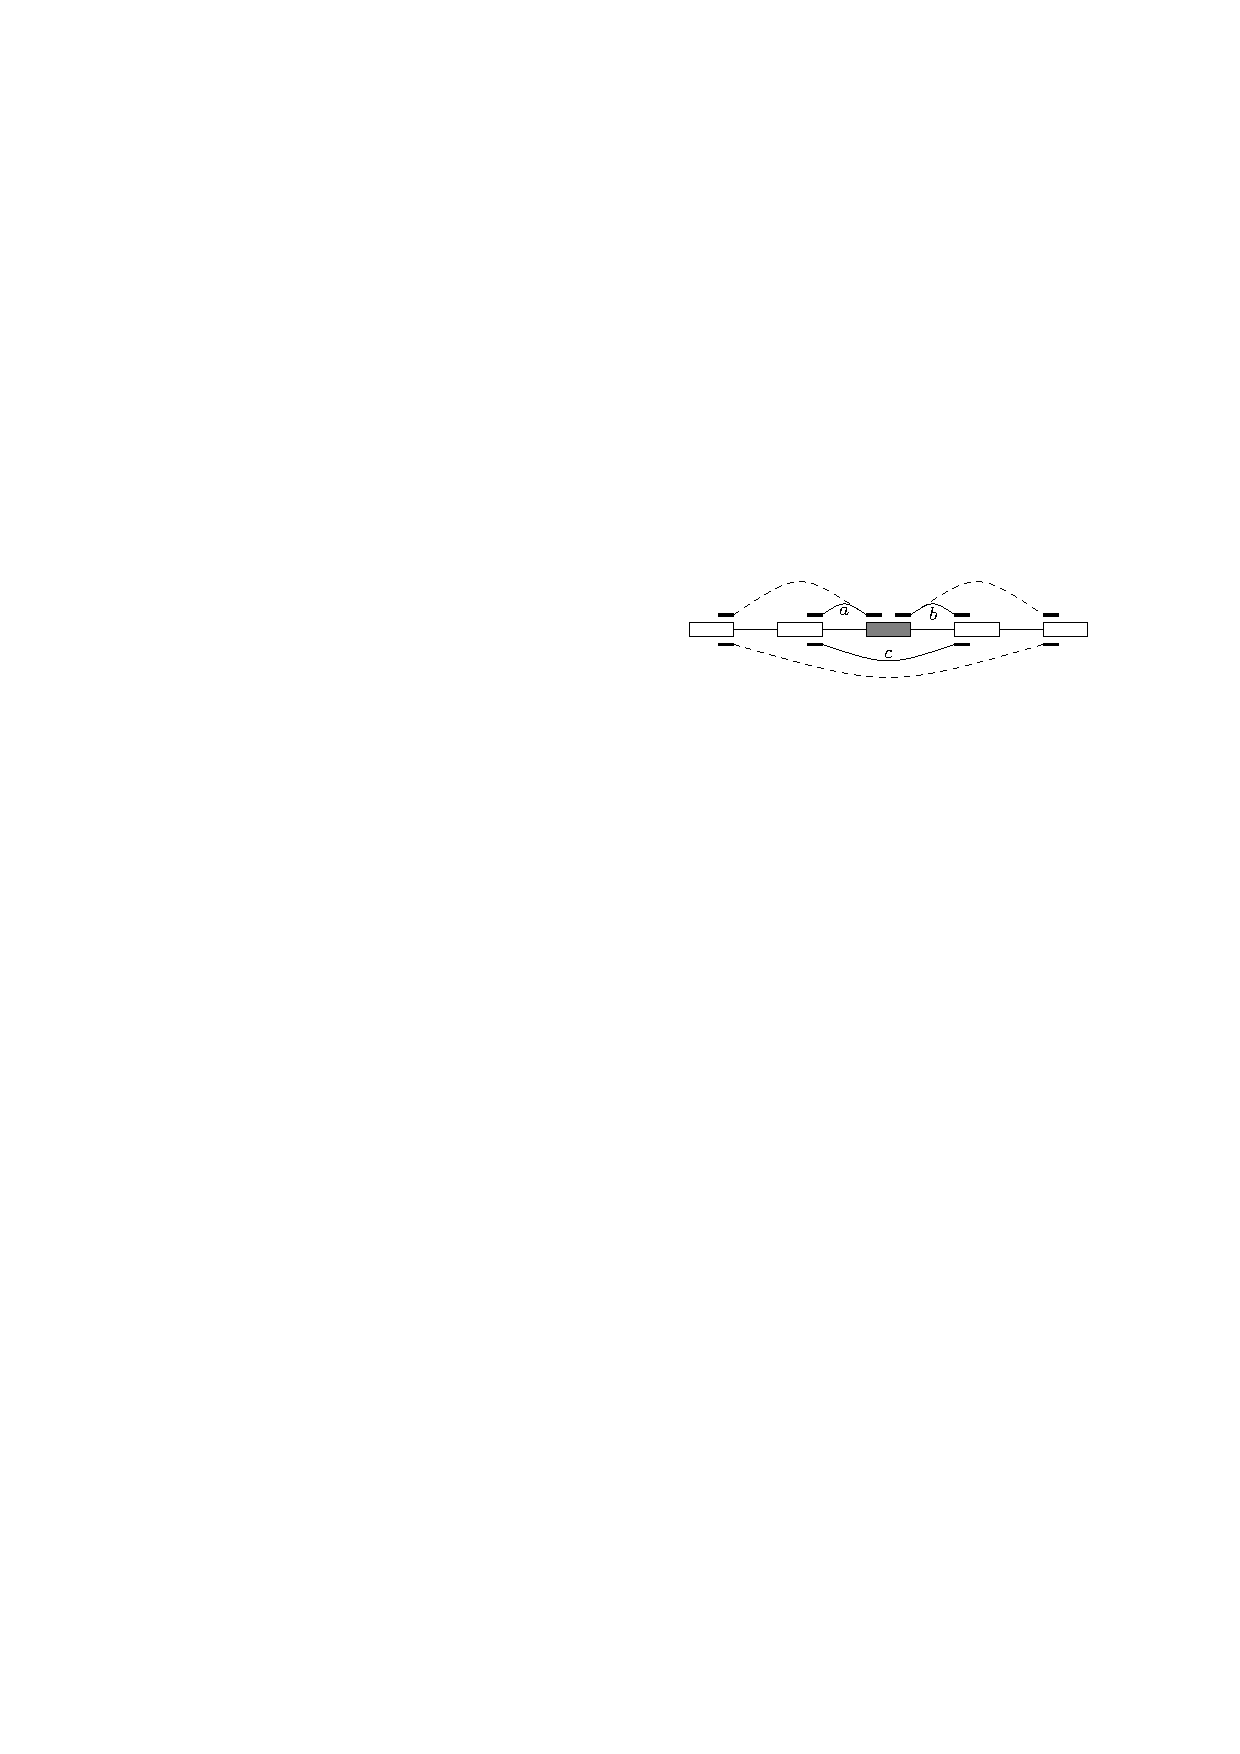
\includegraphics{Latex/psi_def_figure1.pdf}
\caption[Grape-type exonic $\Psi$]{The percent-spliced-in (PSI, $\Psi$) is defined as the number of reads supporting exon inclusion
($a+b$) as the fraction of the combined number of reads supporting inclusion and exclusion ($c$).
The exon of interest if shown in gray.}
\end{center}
\end{figure}
$$\Psi=\frac{a+b}{a+b+2c},\label{eq::psi::eq01}$$

\subsubsection{Intron-centric estimates $\psi_5$, $\psi_3$, $\theta_5$, and  $\theta_3$}
\begin{figure}[h!]
\begin{center}
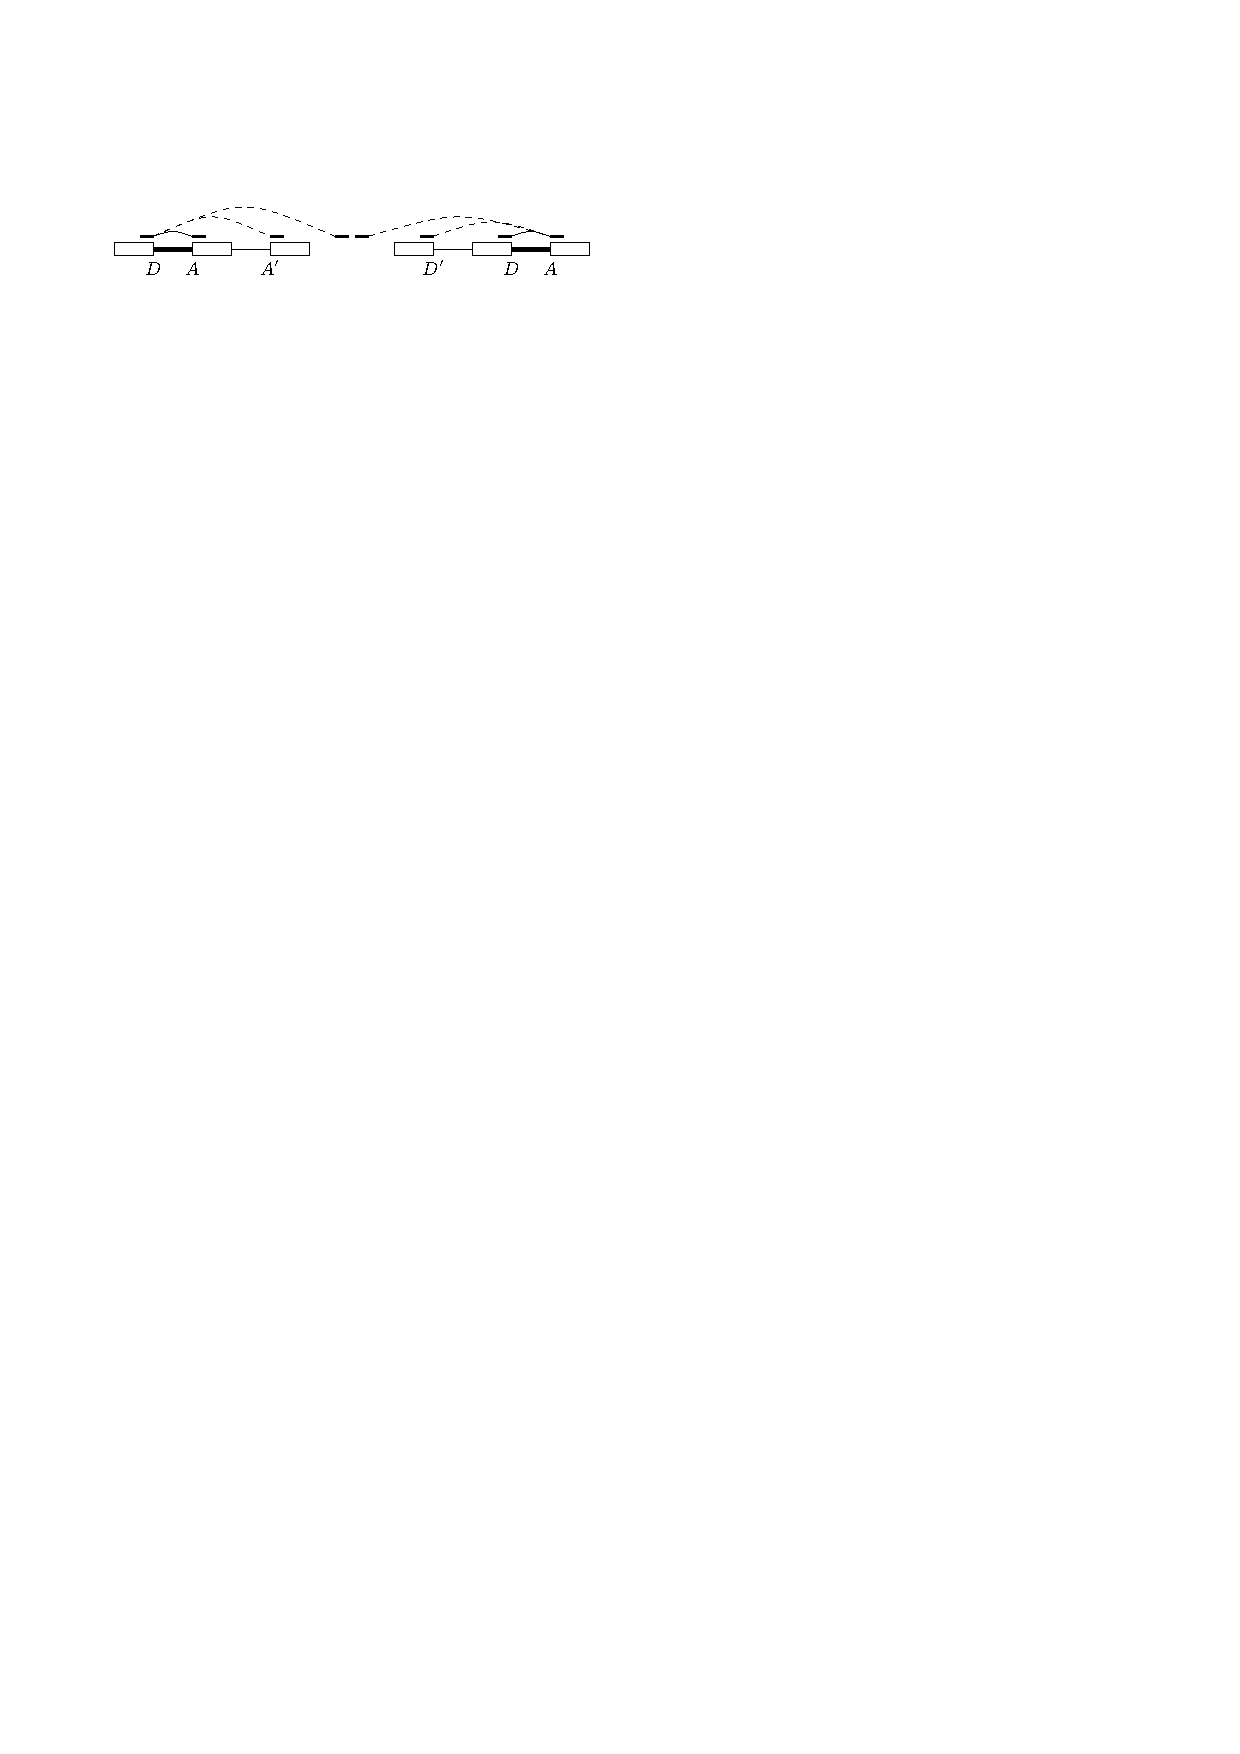
\includegraphics{Latex/psi_def_figure2.pdf}
\caption[Intron-centric estimates $\psi_5$, $\psi_3$, $\theta_5$, and  $\theta_3$]{Left: the 5'-splicing index, $\ii_5$, is the number of reads supporting
the splicing event from $D$ to $A$ relative to the combined number of reads supporting splicing from $D$ to any acceptor site $A'$. 
Right: the 3-splicing index, $\ii_3$, is the number of reads supporting  the splicing event from $D$ to $A$ relative to the combined 
number of reads supporting splicing from any donor site $D'$ to $A$. The intron of interest is drawn thick.}
\end{center}
\end{figure}

$$\ii_5(D,A)=\frac{\nn(D,A)}{\sum\limits_{A'}\nn(D,A')},\quad
\ii_3(D,A)=\frac{\nn(D,A)}{\sum\limits_{D'}\nn(D',A)},\label{eq::psi::eq03}$$
$$\cc_5=\frac{\sum\limits_{A'}\nn(D,A')}{\sum\limits_{A'}\nn(D,A')+\nn(D)},\quad
\cc_3=\frac{\sum\limits_{D'}\nn(D',A)}{\sum\limits_{D'}\nn(D',A)+\nn(A)}.\label{eq::psi::eq05}$$
NB: See section~\ref{sec::comp_exonic_intronic_psi} for the comparison of exonic and intronic estimates

\clearpage


%%%%%%%%%%%%%%%%%%%%%%%%%%%%%%%%%%%%%%%%%%%%%%%%%%%%%%%%%%%%%%%%%%%%%%%%%%%%%%%%%%%%%%%%%%%%%%%%%%%%%%%%%%%%%%
%%%%%%%%%%%%%%%%%%%%%%%%%%%%%%%%%%%%%%%%%%%%%%%%%%%%%%%%%%%%%%%%%%%%%%%%%%%%%%%%%%%%%%%%%%%%%%%%%%%%%%%%%%%%%%
%%%%%%%%%%%%%%%%%%%%%%%%%%%%%%%%%%%%%%%%%%%%%%%%%%%%%%%%%%%%%%%%%%%%%%%%%%%%%%%%%%%%%%%%%%%%%%%%%%%%%%%%%%%%%%
\section{Single-species analysis}
\subsection{Splice site strength}
\subsubsection{Alternative splice sites are, on average, weaker than constitutive ones}
\begin{figure}[h!]
\begin{center}
\subfigure[Human]{\includegraphics[height=5cm,page=1]{output/hg19-strength1.pdf}}%
\subfigure[Mouse]{\includegraphics[height=5cm,page=1]{output/mm9-strength1.pdf}}%
\caption{Strengths of splice sites, by usage }
\end{center}
\end{figure}
\clearpage

\subsubsection{Double-alternative splice sites are even weaker}
\begin{figure}[h!]
\begin{center}
\includegraphics[height=5cm,page=1]{output/hg19-mm9-strength2.pdf}
\caption{Strengths of splice sites, by usage}
\end{center}
\end{figure}
\clearpage

\subsubsection{Pseudogenes have weaker splice sites compared to protein-coding genes and lncRNAs}

\begin{figure}[h!]
\begin{center}
\subfigure[Human]{\includegraphics[height=5cm,page=2]{output/hg19-strength1.pdf}}%
\subfigure[Mouse]{\includegraphics[height=5cm,page=2]{output/mm9-strength1.pdf}}%
\caption{Strengths of splice sites, by biotype }
\end{center}
\end{figure}

\clearpage

\subsection{Mean and variance of $\psi$ and $\theta$}
\subsubsection{In human}
\begin{figure}[h!]
\begin{center}
\subfigure{\includegraphics[height=4cm,page=1]{output/hg19-psi2.pdf}}%
\subfigure{\includegraphics[height=4cm,page=2]{output/hg19-psi2.pdf}}\\
\subfigure{\includegraphics[height=2.5cm,page=3]{output/hg19-psi2.pdf}}%
\subfigure{\includegraphics[height=2.5cm,page=4]{output/hg19-psi2.pdf}}
\caption{Human, $\mean\psi$ and $\Var\psi$ by biotype and vs. $s_D+s_A$}
\end{center}
\end{figure}

\begin{figure}[h!]
\begin{center}
\subfigure{\includegraphics[height=4cm,page=1]{output/hg19-cosi2.pdf}}%
\subfigure{\includegraphics[height=4cm,page=2]{output/hg19-cosi2.pdf}}\\
\subfigure{\includegraphics[height=2.5cm,page=3]{output/hg19-cosi2.pdf}}%
\subfigure{\includegraphics[height=2.5cm,page=4]{output/hg19-cosi2.pdf}}
\caption{Human, $\mean\theta$ and $\Var\theta$ by biotype and vs. $s_D+s_A$}
\end{center}
\end{figure}
\clearpage

\subsubsection{In mouse}
\begin{figure}[h!]
\begin{center}
\subfigure{\includegraphics[height=4cm,page=1]{output/mm9-psi2.pdf}}%
\subfigure{\includegraphics[height=4cm,page=2]{output/mm9-psi2.pdf}}\\
\subfigure{\includegraphics[height=2.5cm,page=3]{output/mm9-psi2.pdf}}%
\subfigure{\includegraphics[height=2.5cm,page=4]{output/mm9-psi2.pdf}}
\caption{Mouse, $\mean\psi$ and $\Var\psi$ by biotype and vs. $s_D+s_A$}
\end{center}
\end{figure}

\begin{figure}[h!]
\begin{center}
\subfigure{\includegraphics[height=4cm,page=1]{output/mm9-cosi2.pdf}}%
\subfigure{\includegraphics[height=4cm,page=2]{output/mm9-cosi2.pdf}}\\
\subfigure{\includegraphics[height=2.5cm,page=3]{output/mm9-cosi2.pdf}}%
\subfigure{\includegraphics[height=2.5cm,page=4]{output/mm9-cosi2.pdf}}
\caption{Mouse, $\mean\theta$ and $\Var\theta$ by biotype and and vs. $s_D+s_A$}
\end{center}
\end{figure}
\clearpage



\subsection{Addendum: logistic transformation}
\label{sec::logistic_transform}
$$\logit(x) = \log_{10}\frac{x}{1-x}$$
\vspace{1cm}
\begin{center}
\begin{tabular}{r|r}
\hline
$x$ & $\logit(x)$\\
\hline
0 & -$\infty$\\
0.001 & -3\\
0.01 & -2\\
0.1 & -1\\
0.5 & 0 \\
0.9 & 1\\
0.99 & 2\\
0.999 & 3\\
1 & +$\infty$\\
\hline
\end{tabular} 
\end{center}
\begin{figure}[h!]
\begin{center}
\subfigure{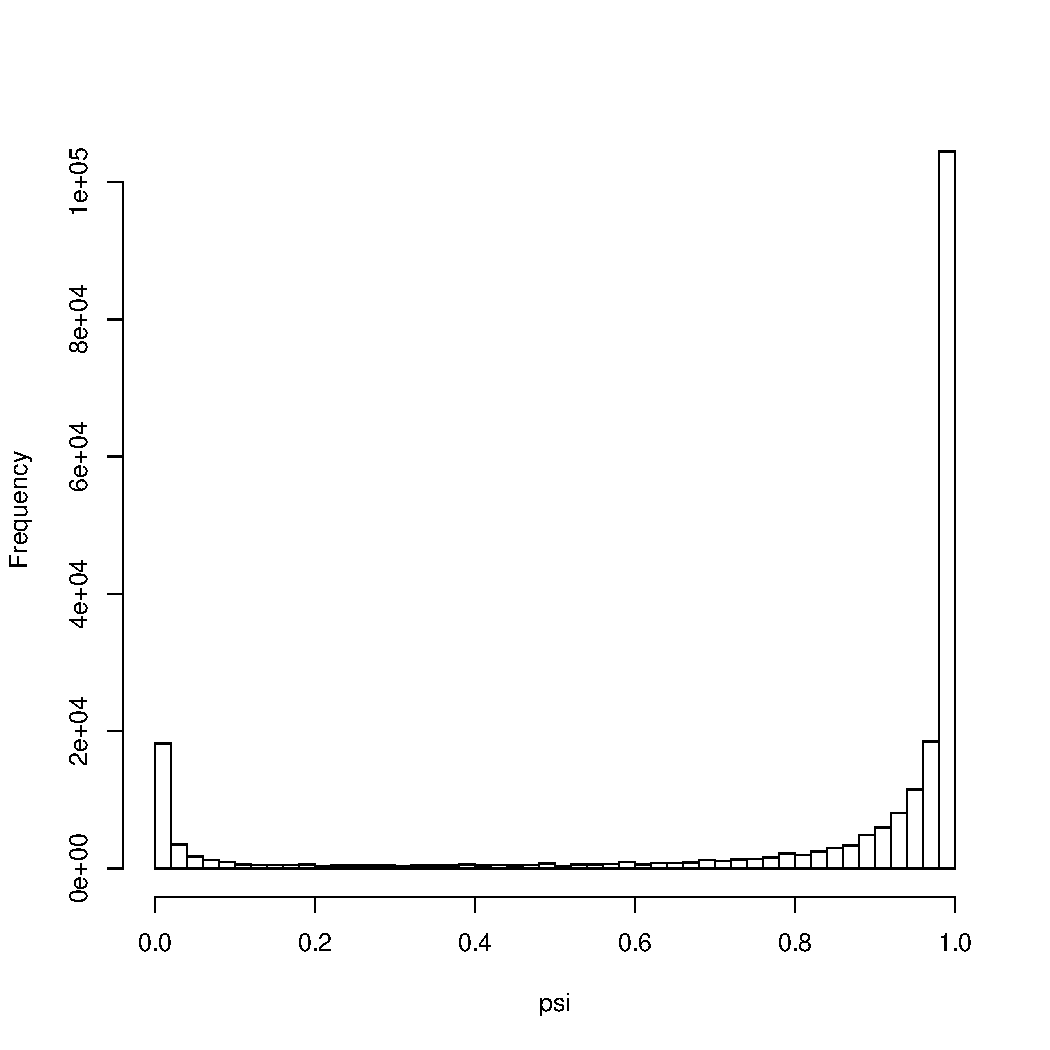
\includegraphics[height=4cm,page=1]{Latex/psi_example.pdf}}%
\subfigure{\includegraphics[height=4cm,page=2]{Latex/psi_example.pdf}}\\
\caption{Distribution of $\psi$ in linear coordinates (left) and logistic coordinates (right)}
\end{center}
\end{figure}
\clearpage

\subsection{Addendum: mean and variance of a Bernoulli variable}
\begin{itemize}
\item $x$ is a Bernoulli variable if $x=0$ with probability $p$ and $x=1$ with probability $1-p$.
\item $\mean(x)=p$ and $\Var(x)=p(1-p)$
\item The closer the mean to 0.5, the greater the variance
\end{itemize}
\clearpage

%%%%%%%%%%%%%%%%%%%%%%%%%%%%%%%%%%%%%%%%%%%%%%%%%%%%%%%%%%%%%%%%%%%%%%%%%%%%%%%%%%%%%%%%%%%%%%%%%%%%%%%%%%%%%%
%%%%%%%%%%%%%%%%%%%%%%%%%%%%%%%%%%%%%%%%%%%%%%%%%%%%%%%%%%%%%%%%%%%%%%%%%%%%%%%%%%%%%%%%%%%%%%%%%%%%%%%%%%%%%%
%%%%%%%%%%%%%%%%%%%%%%%%%%%%%%%%%%%%%%%%%%%%%%%%%%%%%%%%%%%%%%%%%%%%%%%%%%%%%%%%%%%%%%%%%%%%%%%%%%%%%%%%%%%%%%

\section{Cross-species analyses}

\subsection{Definitions}
\begin{itemize}
\item A one-to-one correspondence $f:Human{\to}Mouse$ between splice sites is established (see (a) and (b) below)
\item If $[x,y]$ is a human exon and $f(x)$ and $f(y)$ exist, $[f(x),f(y)]$ might not be annotated as exon in mouse (c)
\begin{center}
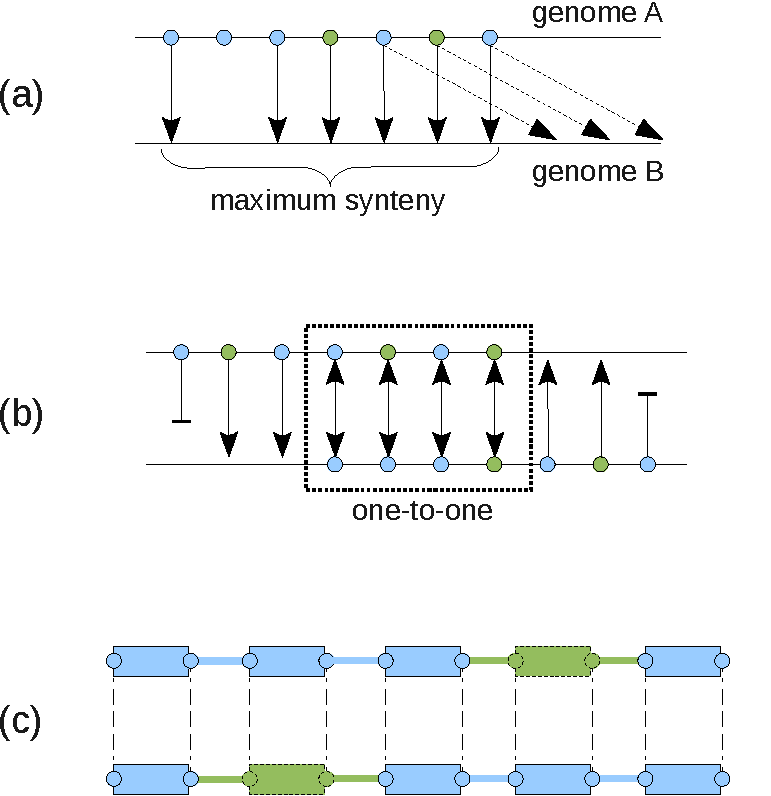
\includegraphics[height=9cm]{Latex/main_legend_2.pdf}
\end{center}
\item additional factor for segments is needed
\begin{itemize}
\item status $\in\{$in human, in mouse, in both$\}$
\end{itemize}
\end{itemize}
\clearpage

\subsection{One-to-one splice sites}
\begin{table}[h!]
\begin{center}
\input{output/hg19.mm9.table3a.tex}
\caption{1-to-1 splice sites, by Biotype}
\end{center}
\end{table}

\begin{table}[h!]
\begin{center}
\input{output/hg19.mm9.table3b.tex}
\caption{1-to-1 splice sites, by Level}
\end{center}
\end{table}

\begin{table}[h!]
\begin{center}
\input{output/hg19.mm9.table3c.tex}
\caption{1-to-1 splice sites, by Usage}
\end{center}
\end{table}

\begin{table}[h!]
\begin{center}
\input{output/hg19.mm9.table3d.tex}
\caption{1-to-1 genes (inferred from splice sites), by Biotype}
\end{center}
\end{table}
\clearpage

\subsection{One-to-one segments}
\begin{table}[h!]
\begin{center}
\input{output/hg19.mm9.table4a.tex}
\caption{1-to-1 segments, by Biotype}
\end{center}
\end{table}

\begin{table}[h!]
\begin{center}
\input{output/hg19.mm9.table4b.tex}
\caption{1-to-1 segments, by Level}
\end{center}
\end{table}

\begin{table}[h!]
\begin{center}
\input{output/hg19.mm9.table4c.tex}
\caption{1-to-1 segments, by Usage}
\end{center}
\end{table}

\begin{table}[h!]
\begin{center}
\input{output/hg19.mm9.table4d.tex}
\caption{1-to-1 segments, by Status}
\end{center}
\end{table}
\clearpage

%%%%%%%%%%%%%%%%%%%%%%%%%%%%%%%%%%%%%%%%%%%%%%%%%%%%%%%%%%%%%%%%%%%%%%%%%%%%%%%%%%%%%%%%%%%%%%%%%%%%%%%%%%%%%%%%%

\subsection{Comparison with e!MIT ortholog list}
\input{output/hg19.mm9.orth1a.tex}
\input{output/hg19.mm9.orth1b.tex}
\clearpage

\subsection{Conservation of usage}
\subsubsection{A splice site is more likely to be alternative if the ortholog is alternative}
\begin{figure}[h!]
\begin{center}
\includegraphics[height=6cm]{output/hg19-mm9-plot3.pdf}
\end{center}
\end{figure}

\subsubsection{Exon or intron is more likely to be alternative if the ortholog is alternative}
\begin{figure}[h!]
\begin{center}
\includegraphics[height=6cm]{output/hg19-mm9-plot4.pdf}
\end{center}
\end{figure}
\clearpage

%%%%%%%%%%%%%%%%%%%%%%%%%%%%%%%%%%%%%%%%%%%%%%%%%%%%%%%%%%%%%%%%%%%%%%%%%%%%%%%%%%%%%%%%%%%%%%%%%%%%%%%%%%%%%%

\newcommand{\diagram}[5]{%
\begin{figure}[h!]
\begin{center}
\subfigure[]{\includegraphics[height=4cm,page=#2]{#1}}%
\subfigure[]{\includegraphics[height=4cm,page=#3]{#1}}%
\subfigure[]{\includegraphics[height=4cm,page=#4]{#1}}
\caption{#5}
\end{center}
\end{figure}
}

\subsection{$\mean(\psi)$ and $\Var(\psi)$ in orthologous genes}
\diagram{output/hg19-mm9-psi.pdf}{2}{10}{17}{Protein coding genes, $\mean(\psi)$, pooled $\psi_5$ and $\psi_3$}
\diagram{output/hg19-mm9-psi.pdf}{6}{14}{18}{Protein coding genes, $\Var(\psi)$, pooled $\psi_5$ and $\psi_3$}
\clearpage

\subsection{Comparison of $\Var(\psi)$ for intron-centric and exon-centric estimates}
\label{sec::comp_exonic_intronic_psi}
\diagram{output/hg19-mm9-psi.pdf}{6}{14}{18}{Protein coding genes, $\Var(\psi)$, pooled $\psi_5$ and $\psi_3$}
\diagram{output/hg19-mm9-psiex.pdf}{6}{14}{18}{Protein coding genes, $\Var(\psi)$, ``grape-style'' $\psi$}
\clearpage

\subsection{$\mean(\theta)$ and $\Var(\theta)$ in orthologous protein coding genes}
\diagram{output/hg19-mm9-cosi.pdf}{2}{10}{17}{Protein coding genes, $\mean(\theta)$, pooled $\psi_5$ and $\psi_3$}
\diagram{output/hg19-mm9-cosi.pdf}{6}{14}{18}{Protein coding genes, $\Var(\theta)$,  pooled $\psi_5$ and $\psi_3$}
\clearpage

%%%%%%%%%%%%%%%%%%%%%%%%%%%%%%%%%%%%%%%%%%%%%%%%%%%%%%%%%%%%%%%%%%%%%%%%%%%%%%%%%%%%%%%%%%%%%%%%%%%%%%%%%%%%%%

\end{document}

